%
% This is sample-sigchi.tex from v1.56 of the ACM Master LaTeX template.
% It has been adjusted to enable content to be inserted into the template
% from the source document main.Rmd, using RStudio
%
% See https://github.com/ulyngs/chi-proc-rmd-template
%
%

\documentclass[sigchi, ]{acmart}

\usepackage{balance} % UL 22 Jan 2019; balance columns on final page, as requested by Lisa M Tolles

\usepackage{booktabs} % For formal tables
\def\tightlist{} % UL 16 Dec 2018 stop pandoc from messing things up by putting lists in 'tightlist' command when no space between bullet points in Rmd file


% UL 19 Dec 2018, enable code inclusion in shaded environments
\usepackage{color}
\usepackage{fancyvrb}
\newcommand{\VerbBar}{|}
\newcommand{\VERB}{\Verb[commandchars=\\\{\}]}
\DefineVerbatimEnvironment{Highlighting}{Verbatim}{commandchars=\\\{\}}
% Add ',fontsize=\small' for more characters per line
\usepackage{framed}
\definecolor{shadecolor}{RGB}{248,248,248}
\newenvironment{Shaded}{\begin{snugshade}}{\end{snugshade}}
\newcommand{\AlertTok}[1]{\textcolor[rgb]{0.94,0.16,0.16}{#1}}
\newcommand{\AnnotationTok}[1]{\textcolor[rgb]{0.56,0.35,0.01}{\textbf{\textit{#1}}}}
\newcommand{\AttributeTok}[1]{\textcolor[rgb]{0.77,0.63,0.00}{#1}}
\newcommand{\BaseNTok}[1]{\textcolor[rgb]{0.00,0.00,0.81}{#1}}
\newcommand{\BuiltInTok}[1]{#1}
\newcommand{\CharTok}[1]{\textcolor[rgb]{0.31,0.60,0.02}{#1}}
\newcommand{\CommentTok}[1]{\textcolor[rgb]{0.56,0.35,0.01}{\textit{#1}}}
\newcommand{\CommentVarTok}[1]{\textcolor[rgb]{0.56,0.35,0.01}{\textbf{\textit{#1}}}}
\newcommand{\ConstantTok}[1]{\textcolor[rgb]{0.00,0.00,0.00}{#1}}
\newcommand{\ControlFlowTok}[1]{\textcolor[rgb]{0.13,0.29,0.53}{\textbf{#1}}}
\newcommand{\DataTypeTok}[1]{\textcolor[rgb]{0.13,0.29,0.53}{#1}}
\newcommand{\DecValTok}[1]{\textcolor[rgb]{0.00,0.00,0.81}{#1}}
\newcommand{\DocumentationTok}[1]{\textcolor[rgb]{0.56,0.35,0.01}{\textbf{\textit{#1}}}}
\newcommand{\ErrorTok}[1]{\textcolor[rgb]{0.64,0.00,0.00}{\textbf{#1}}}
\newcommand{\ExtensionTok}[1]{#1}
\newcommand{\FloatTok}[1]{\textcolor[rgb]{0.00,0.00,0.81}{#1}}
\newcommand{\FunctionTok}[1]{\textcolor[rgb]{0.00,0.00,0.00}{#1}}
\newcommand{\ImportTok}[1]{#1}
\newcommand{\InformationTok}[1]{\textcolor[rgb]{0.56,0.35,0.01}{\textbf{\textit{#1}}}}
\newcommand{\KeywordTok}[1]{\textcolor[rgb]{0.13,0.29,0.53}{\textbf{#1}}}
\newcommand{\NormalTok}[1]{#1}
\newcommand{\OperatorTok}[1]{\textcolor[rgb]{0.81,0.36,0.00}{\textbf{#1}}}
\newcommand{\OtherTok}[1]{\textcolor[rgb]{0.56,0.35,0.01}{#1}}
\newcommand{\PreprocessorTok}[1]{\textcolor[rgb]{0.56,0.35,0.01}{\textit{#1}}}
\newcommand{\RegionMarkerTok}[1]{#1}
\newcommand{\SpecialCharTok}[1]{\textcolor[rgb]{0.00,0.00,0.00}{#1}}
\newcommand{\SpecialStringTok}[1]{\textcolor[rgb]{0.31,0.60,0.02}{#1}}
\newcommand{\StringTok}[1]{\textcolor[rgb]{0.31,0.60,0.02}{#1}}
\newcommand{\VariableTok}[1]{\textcolor[rgb]{0.00,0.00,0.00}{#1}}
\newcommand{\VerbatimStringTok}[1]{\textcolor[rgb]{0.31,0.60,0.02}{#1}}
\newcommand{\WarningTok}[1]{\textcolor[rgb]{0.56,0.35,0.01}{\textbf{\textit{#1}}}}

% Copyright
% \copyrightyear{}
% \acmYear{}
% \setcopyright{}
% \acmConference[]{}{}{}
% \acmBooktitle{}
% \acmPrice{}
% \acmDOI{}
% \acmISBN{}

\settopmatter{printacmref=true}

\begin{document}

\title[]{How to Create Your Own Chunk Options in R Markdown}



\author{Ulrik Lyngs}
\email{}

% The default list of authors is too long for headers.
\renewcommand{\shortauthors}{}


\begin{abstract}

\end{abstract}


\keywords{}



\maketitle

For the \href{http://chi2019.acm.org}{2019 ACM CHI conference} I wanted to go all in on reproducibility and write our paper submission completely in R Markdown, and just tweak the ACM's LaTeX template so that I could use it as a template for R Markdown to use when outputting to PDF.
It worked in the end (find PDF pre-print and .Rmd source file for our paper \href{https://osf.io/zyj4h/}{here}, an R package that makes it easy \href{https://github.com/ulyngs/chi-proc-rmd-template}{here}, and a blog post about the process \href{https://ulyngs.github.io/blog/posts/2018-10-28-how-to-write-acm-articles-with-r-markdown/}{here}), but along the way I found that I was missing some chunk options to be able to keep my paper reproducible.

For example, in an update to their LaTeX template, the ACM now wanted all figures to include a description to improve accessibility for visually impaired readers.
In LaTeX, this was supposed to be accomplished by adding \texttt{\textbackslash{}Description\{This\ is\ a\ figure\ description\}} inside the relevant figure environment.
How should I handle this while staying within my R Markdown-based workflow?

One option would be to add these descriptions manually in LaTeX as the last step before finishing the paper - that is, I could add \texttt{keep\_tex:\ true} in my YAML header, then manually adjust the \textbf{.tex} file for our paper and then re-generate a PDF from this LaTeX file.
This would work but it was also a bad option that would be error-prone: if I discovered some mistake that would need fixing in the R Markdown source file and require me to recompile and re-create the \textbf{.tex} file, then I would have to add all the descriptions again\ldots{}

The much better solution would be if there simply existed a chunk option `description' that I could set directly in the R Markdown source file with something like `\texttt{\textasciigrave{}\textasciigrave{}\textasciigrave{}\{r\ my\_figure,\ description="This\ is\ a\ figure\ description"\}}, and which would then automatically add \texttt{\textbackslash{}Description\{This\ is\ a\ figure\ description\}} when knitting to PDF. Fortunately, it is possible to just create new chunk options yourself!

\hypertarget{getting-a-grip-on-knit-output-hooks}{%
\section{Getting a grip on knit output hooks}\label{getting-a-grip-on-knit-output-hooks}}

\href{https://yihui.name/knitr/}{Knitr}, which does the first part of R Markdown's work under the hood, provides `hooks' which are \href{https://yihui.name/knitr/hooks/}{``customisable functions to run before/after a code chunk, tweak the output, and manipulate chunk options''}. We will work with `output hooks' which are used to customise and polish \emph{raw} output from chunks. There are 8 different kinds of output hooks that can grab different types of output; for our purpose we will modify the \texttt{chunk} output hook which grab all the output of a chunk.

A chunk output hook takes the form \texttt{function\ (x,\ options)} where \texttt{x} is a character string of the output and \texttt{options} is a list of the chunk options.

To modify them, do this:

\begin{Shaded}
\begin{Highlighting}[]
\NormalTok{knit_hooks}\OperatorTok{$}\KeywordTok{set}\NormalTok{(}\DataTypeTok{chunk =} \ControlFlowTok{function}\NormalTok{(x, options) \{}
  \CommentTok{# some code to modify chunk output hooks here}
\NormalTok{\})}
\end{Highlighting}
\end{Shaded}

\hypertarget{the-stupidest-possible-thing-to-do}{%
\subsection{The stupidest possible thing to do}\label{the-stupidest-possible-thing-to-do}}

The stupidest possible thing we might do do would be to get all chunks to output ``Hello, world!''.

Here is a random plot:

\begin{Shaded}
\begin{Highlighting}[]
\KeywordTok{plot}\NormalTok{(pressure)}
\end{Highlighting}
\end{Shaded}

\begin{figure}
\centering
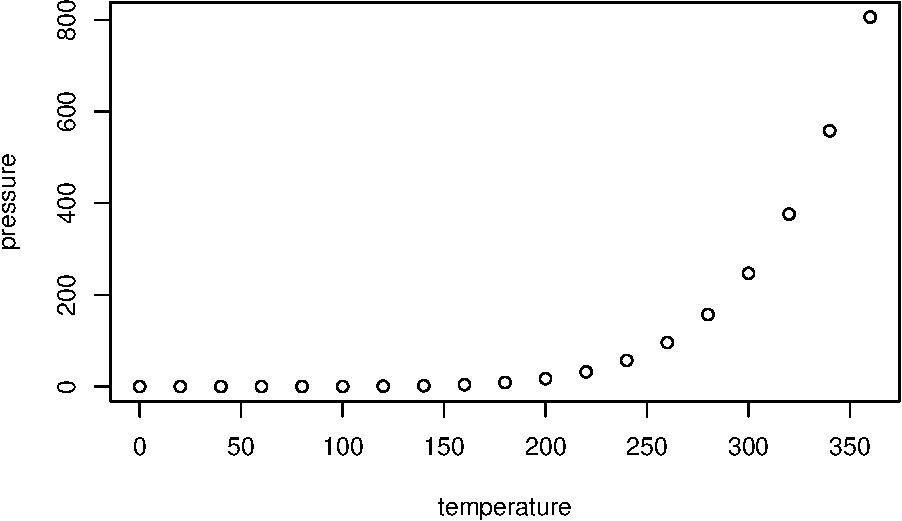
\includegraphics{how-to-create-your-own-chunk-options-in-r-markdown_files/figure-latex/random-plot-1.pdf}
\caption{\label{fig:random-plot}A random plot}
\end{figure}

Then we modify the chunk output hook to return `hello world':
First, let's store the current configuration of the chunk output hook, and have a look at it as well:

\begin{verbatim}
## function (x, options) 
## {
##     x = gsub(paste0("[\n]{2,}(", fence, "|    )"), "\n\n\\1", 
##         x)
##     x = gsub("[\n]+$", "", x)
##     x = gsub("^[\n]+", "\n", x)
##     if (isTRUE(options$collapse)) {
##         x = gsub(paste0("\n([", fence_char, "]{3,})\n+\\1(", 
##             tolower(options$engine), ")?\n"), "\n", x)
##     }
##     if (is.null(s <- options$indent)) 
##         return(x)
##     line_prompt(x, prompt = s, continue = s)
## }
## <bytecode: 0x7f88d16720e8>
## <environment: 0x7f88d16842e0>
\end{verbatim}

Then modify it:

\begin{Shaded}
\begin{Highlighting}[]
\NormalTok{knit_hooks}\OperatorTok{$}\KeywordTok{set}\NormalTok{(}\DataTypeTok{chunk =} \ControlFlowTok{function}\NormalTok{(x, options) \{}
  \KeywordTok{return}\NormalTok{(}\StringTok{"Hello, world!"}\NormalTok{)}
\NormalTok{\})}
\end{Highlighting}
\end{Shaded}

Now if we try do draw the random plot again we simply get:

Hello, world!

\hypertarget{creating-a-new-chunk-option}{%
\subsection{Creating a new chunk option}\label{creating-a-new-chunk-option}}

To make this minimally more useful, imagine if this only happened if we set a chunk option \texttt{hello}.

Let's first set the output hook back to what it was:

\begin{Shaded}
\begin{Highlighting}[]
\NormalTok{knit_hooks}\OperatorTok{$}\KeywordTok{set}\NormalTok{(}\DataTypeTok{chunk =}\NormalTok{ hook_chunk)}
\end{Highlighting}
\end{Shaded}

Now let's modify it again:

\begin{Shaded}
\begin{Highlighting}[]
\NormalTok{knit_hooks}\OperatorTok{$}\KeywordTok{set}\NormalTok{(}\DataTypeTok{chunk =} \ControlFlowTok{function}\NormalTok{(x, options) \{}
  \ControlFlowTok{if}\NormalTok{ (}\OperatorTok{!}\KeywordTok{is.null}\NormalTok{(options}\OperatorTok{$}\NormalTok{hello)) \{}
    \KeywordTok{return}\NormalTok{(}\StringTok{"Hello, world!"}\NormalTok{)}
\NormalTok{  \} }\ControlFlowTok{else}\NormalTok{ \{}
    \KeywordTok{return}\NormalTok{(}\KeywordTok{hook_chunk}\NormalTok{(x, options))}
\NormalTok{  \}}
\NormalTok{\})}
\end{Highlighting}
\end{Shaded}

Let's check if this works. Here's our random plot again (Figure \ref{fig:random-plot-no-hello}):

\begin{Shaded}
\begin{Highlighting}[]
\KeywordTok{plot}\NormalTok{(pressure)}
\end{Highlighting}
\end{Shaded}

\begin{figure}
\centering
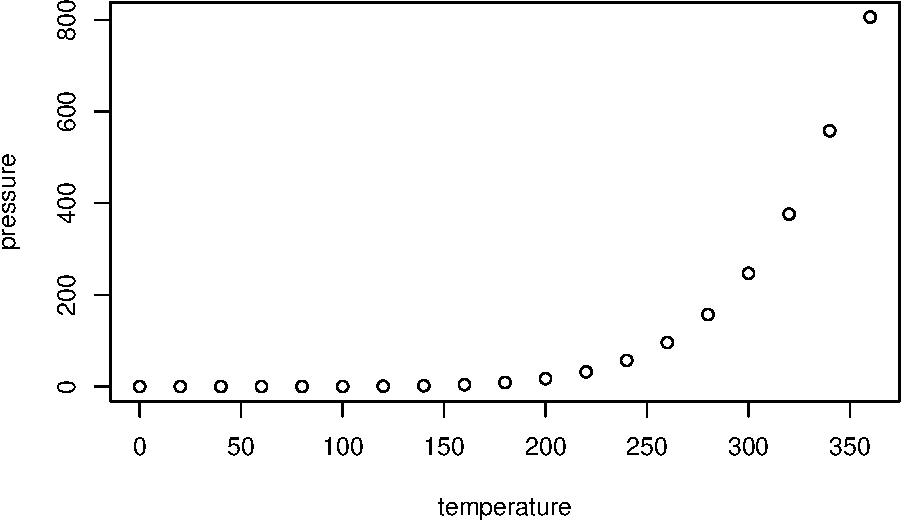
\includegraphics{how-to-create-your-own-chunk-options-in-r-markdown_files/figure-latex/random-plot-no-hello-1.pdf}
\caption{\label{fig:random-plot-no-hello}A random plot}
\end{figure}

And here it is with chunk option \texttt{hello=TRUE}:
Hello, world!

\hypertarget{example-use-adding-description-to-latex-figure-output}{%
\section{Example use: Adding \textbackslash{}Description\{\} to LaTeX figure output}\label{example-use-adding-description-to-latex-figure-output}}

Finally, let's create an actually useful chunk option: the option to add a \texttt{\textbackslash{}Description\{\}} to figures in PDF output, which is what I needed. For good measure, let's start by resetting the chunk output hook to its original state:

\begin{Shaded}
\begin{Highlighting}[]
\NormalTok{knit_hooks}\OperatorTok{$}\KeywordTok{set}\NormalTok{(}\DataTypeTok{chunk =}\NormalTok{ hook_chunk)}
\end{Highlighting}
\end{Shaded}

The problem we're trying to solve is this: If we knit to PDF and set \texttt{keep\_tex\ =\ TRUE} in the YAML header, we see that our random plot included in the \textbf{.tex} file in this way:

\begin{Shaded}
\begin{Highlighting}[]
\KeywordTok{\textbackslash{}begin}\NormalTok{\{}\ExtensionTok{figure}\NormalTok{\}}
\FunctionTok{\textbackslash{}centering}
\BuiltInTok{\textbackslash{}includegraphics}\NormalTok{\{}\ExtensionTok{how-to-create-your-own-chunk-options-in-r-markdown_files/figure-latex/random-plot-1.pdf}\NormalTok{\}}
\FunctionTok{\textbackslash{}caption}\NormalTok{\{A random plot\}}
\KeywordTok{\textbackslash{}end}\NormalTok{\{}\ExtensionTok{figure}\NormalTok{\}}
\end{Highlighting}
\end{Shaded}

What we want in our \textbf{.tex} file is this:

\begin{Shaded}
\begin{Highlighting}[]
\KeywordTok{\textbackslash{}begin}\NormalTok{\{}\ExtensionTok{figure}\NormalTok{\}}
\FunctionTok{\textbackslash{}centering}
\BuiltInTok{\textbackslash{}includegraphics}\NormalTok{\{}\ExtensionTok{how-to-create-your-own-chunk-options-in-r-markdown_files/figure-latex/random-plot-1.pdf}\NormalTok{\}}
\FunctionTok{\textbackslash{}Description}\NormalTok{\{A scatter plot of an exponentially growing curve\}}
\FunctionTok{\textbackslash{}caption}\NormalTok{\{A random plot\}}
\KeywordTok{\textbackslash{}end}\NormalTok{\{}\ExtensionTok{figure}\NormalTok{\}}
\end{Highlighting}
\end{Shaded}

We would like this to be easily done via a chunk option \texttt{description}. What we want to do is search through the usual LaTeX output with a \href{https://r4ds.had.co.nz/strings.html\#matching-patterns-with-regular-expressions}{regular expression} and insert \texttt{\textbackslash{}Description\{A\ scatter\ plot\ of\ an\ exponentially\ growing\ curve\}} after the call to \texttt{\textbackslash{}includegraphics}.

Note that if you want to follow along with this example, you must output to PDF via an ACM LaTeX template in which \texttt{Description} has been defined as a control sequence. If you go to \href{https://github.com/ulyngs/chi-proc-rmd-template}{github.com/ulyngs/chi-proc-rmd-template} you will find the relevant files in \textbf{chi-proc-rmd-template/inst/rmarkdown/templates/acm\_chi\_proc/skeleton/}.

This should work:

\begin{Shaded}
\begin{Highlighting}[]
\CommentTok{# store the usual chunk output function}
\NormalTok{hook_chunk =}\StringTok{ }\NormalTok{knit_hooks}\OperatorTok{$}\KeywordTok{get}\NormalTok{(}\StringTok{'chunk'}\NormalTok{)}

\NormalTok{knit_hooks}\OperatorTok{$}\KeywordTok{set}\NormalTok{(}\DataTypeTok{chunk =} \ControlFlowTok{function}\NormalTok{(x, options) \{}
\NormalTok{  regular_output =}\StringTok{ }\KeywordTok{hook_chunk}\NormalTok{(x, options)}

  \CommentTok{# if there is a description}
  \ControlFlowTok{if}\NormalTok{ (}\OperatorTok{!}\KeywordTok{is.null}\NormalTok{(options}\OperatorTok{$}\NormalTok{description)) \{}
    \CommentTok{# include the following LaTeX - \textbackslash{}\textbackslash{}1 refers to the regex grouping}
\NormalTok{    latex_include <-}\StringTok{ }\KeywordTok{paste0}\NormalTok{(}\StringTok{"}\CharTok{\textbackslash{}\textbackslash{}}\StringTok{1}\CharTok{\textbackslash{}\textbackslash{}\textbackslash{}\textbackslash{}}\StringTok{Description}\CharTok{\textbackslash{}\textbackslash{}}\StringTok{\{"}\NormalTok{, options}\OperatorTok{$}\NormalTok{description, }\StringTok{"}\CharTok{\textbackslash{}\textbackslash{}}\StringTok{\}"}\NormalTok{)}
    
    \CommentTok{# search and replace in the output}
    \KeywordTok{gsub}\NormalTok{(}\StringTok{'(}\CharTok{\textbackslash{}\textbackslash{}\textbackslash{}\textbackslash{}}\StringTok{includegraphics[^\}]+\})'}\NormalTok{, latex_include, regular_output) }
    
\NormalTok{  \} }\ControlFlowTok{else}\NormalTok{ \{}
    
    \CommentTok{# if there isn't a description just return unmodified}
    \KeywordTok{return}\NormalTok{(regular_output)  }\CommentTok{# pass to default hook}
    
\NormalTok{  \}}
\NormalTok{\})}
\end{Highlighting}
\end{Shaded}

So now let's try with these chunk options for Figure \ref{fig:my-description}:

\texttt{\textasciigrave{}\textasciigrave{}\textasciigrave{}\{r\ my-description,\ echo=TRUE,\ fig.cap="A\ random\ plot",\ description="A\ scatter\ plot\ of\ an\ exponentially\ growing\ curve"\}}

\begin{Shaded}
\begin{Highlighting}[]
\KeywordTok{plot}\NormalTok{(pressure)}
\end{Highlighting}
\end{Shaded}

\begin{figure}
\centering
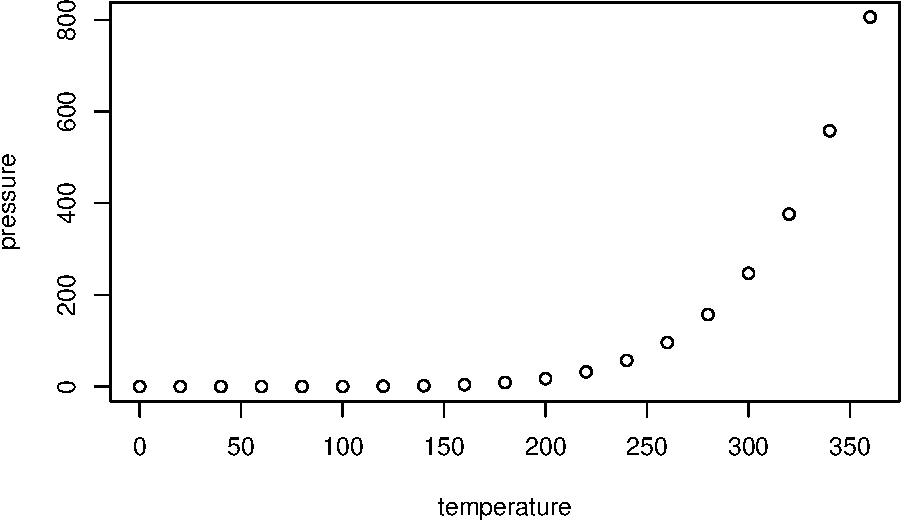
\includegraphics{how-to-create-your-own-chunk-options-in-r-markdown_files/figure-latex/my-description-1.pdf}
\caption{\label{fig:my-description}A random plot}
\end{figure}

Uh-oh it actually doesn't work, our LaTeX output still shows like this:

Turns out that for this to work we have to be explicit with \textbf{knitr} that the figure output is intended to be treated as LaTeX when we're trying to modify output (see Yihui Xie's explanation for why here: \href{https://github.com/yihui/knitr/issues/1464}{github.com/yihui/knitr/issues/1464}).

So when we want to modify LaTeX output in our R Markdown document, we need to add this in out setup chunk:

\begin{Shaded}
\begin{Highlighting}[]
\ControlFlowTok{if}\NormalTok{ (knitr}\OperatorTok{::}\KeywordTok{is_latex_output}\NormalTok{()) knitr}\OperatorTok{::}\NormalTok{knit_hooks}\OperatorTok{$}\KeywordTok{set}\NormalTok{(}\DataTypeTok{plot =}\NormalTok{ knitr}\OperatorTok{::}\NormalTok{hook_plot_tex)}
\end{Highlighting}
\end{Shaded}

Let's try again:

\begin{Shaded}
\begin{Highlighting}[]
\KeywordTok{plot}\NormalTok{(pressure)}
\end{Highlighting}
\end{Shaded}

\begin{figure}
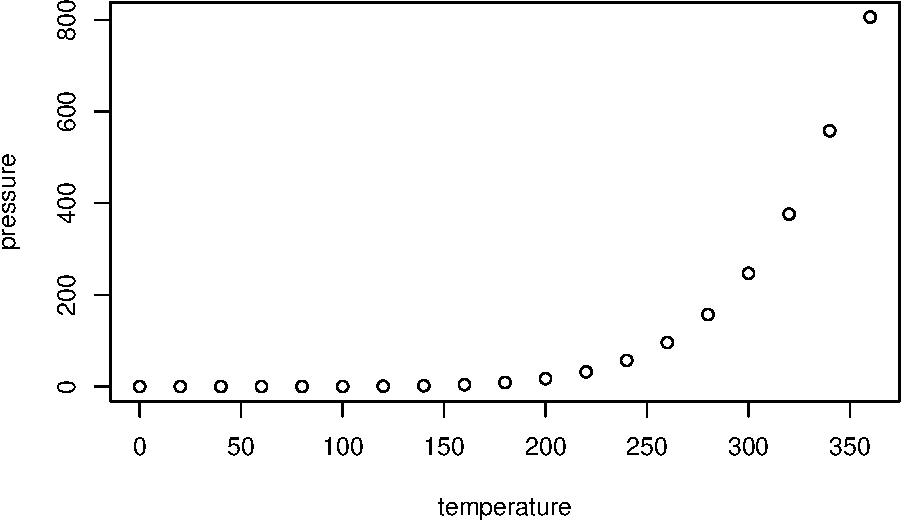
\includegraphics{how-to-create-your-own-chunk-options-in-r-markdown_files/figure-latex/my-description-correct-1}\Description{A scatter plot of an exponentially growing curve} \caption[A random plot]{A random plot}\label{fig:my-description-correct}
\end{figure}

Yup the LaTeX generated for Figure \ref{fig:my-description-correct} now looks as we wanted:

\begin{Shaded}
\begin{Highlighting}[]
\KeywordTok{\textbackslash{}begin}\NormalTok{\{}\ExtensionTok{figure}\NormalTok{\}}
\BuiltInTok{\textbackslash{}includegraphics}\NormalTok{\{}\ExtensionTok{how-to-create-your-own-chunk-options-in-r-markdown_files/figure-latex/my-description-1}\NormalTok{\}}\FunctionTok{\textbackslash{}Description}\NormalTok{\{yeah\} }\FunctionTok{\textbackslash{}caption}\NormalTok{\{A random plot\}}\KeywordTok{\textbackslash{}label}\NormalTok{\{}\ExtensionTok{fig:my-description}\NormalTok{\}}
\KeywordTok{\textbackslash{}end}\NormalTok{\{}\ExtensionTok{figure}\NormalTok{\}}
\end{Highlighting}
\end{Shaded}

\hypertarget{conclusion}{%
\section{Conclusion}\label{conclusion}}

It is super powerful to be able to define your own chunk options. In the R Markdown template for CHI proceedings, I also create a chunk option that allows chunks to be positioned vertically in PDF output by inserting the LaTeX commmand \texttt{\textbackslash{}vspace}, so that the relevant part of the initial setup chunk looks like this:

\begin{Shaded}
\begin{Highlighting}[]
\CommentTok{# create additional chunk options}
\NormalTok{hook_chunk =}\StringTok{ }\NormalTok{knit_hooks}\OperatorTok{$}\KeywordTok{get}\NormalTok{(}\StringTok{'chunk'}\NormalTok{)}
\NormalTok{knit_hooks}\OperatorTok{$}\KeywordTok{set}\NormalTok{(}\DataTypeTok{chunk =} \ControlFlowTok{function}\NormalTok{(x, options) \{}
\NormalTok{  txt =}\StringTok{ }\KeywordTok{hook_chunk}\NormalTok{(x, options)}
  \CommentTok{# add chunk option 'vspaceout' to position chunks vertically with \textbackslash{}vspace}
  \ControlFlowTok{if}\NormalTok{ (}\OperatorTok{!}\KeywordTok{is.null}\NormalTok{(options}\OperatorTok{$}\NormalTok{vspaceout)) \{}
\NormalTok{    latex_vspace <-}\StringTok{ }\KeywordTok{paste0}\NormalTok{(}\StringTok{"}\CharTok{\textbackslash{}\textbackslash{}}\StringTok{1}\CharTok{\textbackslash{}\textbackslash{}\textbackslash{}\textbackslash{}}\StringTok{vspace}\CharTok{\textbackslash{}\textbackslash{}}\StringTok{\{"}\NormalTok{, options}\OperatorTok{$}\NormalTok{vspaceout, }\StringTok{"}\CharTok{\textbackslash{}\textbackslash{}}\StringTok{\}"}\NormalTok{)}
\NormalTok{    txt <-}\StringTok{ }\KeywordTok{sub}\NormalTok{(}\StringTok{'(}\CharTok{\textbackslash{}\textbackslash{}\textbackslash{}\textbackslash{}}\StringTok{begin[^\}]+\})'}\NormalTok{, latex_vspace, txt)  }
\NormalTok{  \}}
  \CommentTok{# add chunk option 'description' which adds \textbackslash{}Description\{...\} to figures}
  \ControlFlowTok{if}\NormalTok{ (}\OperatorTok{!}\KeywordTok{is.null}\NormalTok{(options}\OperatorTok{$}\NormalTok{description)) \{}
\NormalTok{    latex_include <-}\StringTok{ }\KeywordTok{paste0}\NormalTok{(}\StringTok{"}\CharTok{\textbackslash{}\textbackslash{}}\StringTok{1}\CharTok{\textbackslash{}\textbackslash{}\textbackslash{}\textbackslash{}}\StringTok{Description}\CharTok{\textbackslash{}\textbackslash{}}\StringTok{\{"}\NormalTok{, options}\OperatorTok{$}\NormalTok{description, }\StringTok{"}\CharTok{\textbackslash{}\textbackslash{}}\StringTok{\}"}\NormalTok{)}
    \KeywordTok{gsub}\NormalTok{(}\StringTok{'(}\CharTok{\textbackslash{}\textbackslash{}\textbackslash{}\textbackslash{}}\StringTok{includegraphics[^\}]+\})'}\NormalTok{, latex_include, txt) }
\NormalTok{  \} }\ControlFlowTok{else}\NormalTok{ \{}
    \KeywordTok{return}\NormalTok{(txt)  }\CommentTok{# pass to default hook}
\NormalTok{  \}}
\NormalTok{\})}
\end{Highlighting}
\end{Shaded}

You can inspect this in context \href{https://github.com/ulyngs/chi-proc-rmd-template/blob/master/inst/rmarkdown/templates/acm_chi_proc/skeleton/skeleton.Rmd}{here}. Now go ahead and put your newfound customisation powers into practice!

\bibliographystyle{ACM-Reference-Format}
\balance
\bibliography{}

\end{document}
